% Section content template for individual Educative lessons
% This file contains the actual content for a specific section
% Generated from Educative API section content

% Section: Requirements of Uber’s Design
% Section ID: 6376322179268608
% Section Slug: requirements-of-ubers-design
% Generated: 2025-12-07T23:30:30.709859

\subsection{Requirements}\label{il2d43JNa_obTDtmmPFUV}
\\
Let's start with the requirements for designing a system like Uber.

\subsubsection{Functional requirements}\label{ibir-FW8M1oyMeeBjQ3F8}
\\
The functional requirements of our system are as follows:

\begin{itemize}
\item
\protect\phantomsection\label{jFlEI8AG2YR8OIyg4Vrv7}
\textbf{Update driver location}: The driver is a moving entity, so the driver's location should be automatically updated at regular intervals.
\item
\protect\phantomsection\label{LPYd-OiWZyI8EOf-RAzAd}
\textbf{Find nearby drivers}: The system should find and show the nearby available drivers to the rider.
\end{itemize}
\\
\textbf{Note:} Drivers can be ranked not only by proximity but also by ratings, popularity, or other relevance metrics to optimize matching.

\begin{itemize}
\item
\protect\phantomsection\label{kcLPe-nR_SitUiTHBB12l}
\textbf{Request a ride}: A rider should be able to request a ride, after which the nearest driver should be notified about the rider's request.
\item
\protect\phantomsection\label{00SUEEYEuU70c0g3_fqFj}
\textbf{Manage payments:} At the start of the trip, the system must initiate the payment process and manage the payments.
\item
\protect\phantomsection\label{qLK75tZqSg6utr9sfthyz}
\textbf{Show driver estimated time of arrival (ETA):} The rider should be able to see the estimated time of arrival of the driver.
\item
\protect\phantomsection\label{9gIgpbRyURfmmLasPzfyO}
\textbf{Confirm pickup:} Drivers should be able to confirm that they have picked up the rider.
\item
\protect\phantomsection\label{fwKYW_eN5Wj6EuNDVd8FA}
\textbf{Show trip updates}: Once a driver and a rider accept a ride, they should be able to constantly see trip updates like ETA and current location until the trip finishes.
\item
\protect\phantomsection\label{LBOrIegEBx4aPuzPVmZ3N}
\textbf{End the trip:} The driver marks the journey complete upon reaching the destination, and they then become available for the next ride.
\item
\protect\phantomsection\label{bjHLhWYNdJ9YFzTcfeQvY}
\textbf{Notifications}: The system should push location updates and ride requests to relevant customers and drivers in real-time, using a publisher-subscriber notification model or a pull mechanism for dynamic areas.
\end{itemize}
\\
\textbf{You might be wondering:} What if two drivers are at the same distance from the rider?\\
Let's think it through before moving on.
\\
How should the system decide which driver gets the ride request?

\textbf{Question:}

What if two drivers are at the same distance from the rider? How will we select the driver to whom we'll send the request?

\textbf{Reference Answer:}

This decision will be made on multiple factors, such as the distance, type of vehicle, rank of the driver, and so on. Still , if two drivers are identical, we can randomly select one and send a request to that driver. If one driver doesn't accept the ride within a few seconds, we retract the ride offer from this driver and present it to a new one.

\subsubsection{Non-functional requirements}\label{ZHOw7xVdh1rCBj1Mu27G0}
\\
The non-functional requirements of our system are as follows:

\begin{itemize}
\item
\protect\phantomsection\label{7ESv-SWI3Mj40s3lb5UF6}
\textbf{Availability:} The system should be highly available. The downtime of even a fraction of a second can result in a trip failure, with the driver being unable to locate the rider or the rider being unable to contact the driver.
\item
\protect\phantomsection\label{wQarkrFXQLuwIoE8qJauE}
\textbf{Scalability:} The system should be scalable to handle an ever-increasing number of drivers and riders over time.
\item
\protect\phantomsection\label{wsAEOZTGsEkKdFUUrYnb8}
\textbf{Reliability:} The system should provide fast and error-free services. Ride requests and location updates should happen smoothly.
\item
\protect\phantomsection\label{XOgWOaD0sQ4Otrbv83T6z}
\textbf{Consistency:} The system must be strongly consistent. The drivers and riders in an area should have a consistent view of the system.
\item
\protect\phantomsection\label{zOjE2wLXx8RkMVJ7Of_Rv}
\textbf{Fraud detection:} The system should have the ability to detect any fraudulent activity related to payment.
\end{itemize}

\subsection{Resource estimation}\label{cNrd_UH5DCl82jczIUCxv}
\\
Now, let's estimate the resources for our design. Let 's assume it has around 500 million riders and about five million drivers. We
'll assume the following numbers for our estimates:

\begin{itemize}
\item
\protect\phantomsection\label{aF0aZCaz9a8wyVveBj7q5}
We have 20 million daily active riders and three million daily active drivers.
\item
\protect\phantomsection\label{D7sRRzrLmQev68xzxuv_R}
We have 20 million daily trips.
\item
\protect\phantomsection\label{g9BNBTOhMZzqgHg8tgGGj}
All active drivers send a notification of their current location every four seconds.
\end{itemize}

\subsubsection{Storage estimation}\label{uTHp4g_jnK-wwSeG3Mmf0}
\\
Let's estimate the storage required for our system:
\\
\paragraph{Rider's metadata}\label{_whAKXbQ5SLicewQGbX5-}
\\
Let's assume we need around 1,000 Bytes to store each rider's information, including ID, name, email, and so on, when the rider registers in our application. To store the 500 million riders, we require 500 GB of storage:

\[
{500 \times 10^6 \times 1000 } = 500\ \text{GB}
\]

Additionally, if we have around 500,000 new riders registered daily, we'll need a further 500 MB to store them.\\
\\
\paragraph{Driver's metadata}\label{wE1YprEZpyc47kkYr2onc}
\\
\hfill\break
Let's assume we need around 1,000 Bytes to store each driver's information, including ID, name, email, vehicle type, and so on, when the driver registers in our application. To store the five million drivers, we require 5 GB of storage:

\[
{5 \times 10^6 \times 1000 } = 5\ \text{GB}
\]

Additionally, if we have around 100,000 new drivers registered daily, we'll need around 100 MB to store them.\\
\strut \\
\strut \\
\\
\paragraph{Driver location metadata}\label{DHeUVDCtOgOL-dYEkg0qx}
\\
Let's assume we need around 36 Bytes to store the driver's location updates. If we have three million drivers, we need around 108 MB of storage just for the drivers' locations.
\\
\paragraph{Trip metadata}\label{tN-VJ9VhSNz4Xs14qBioQ}
\\
Let's assume we need around 100 Bytes to store single-trip information, including trip ID, rider ID, driver ID, and so on. If we have 20 million daily rides, we need around 2 GB of storage for the trip data.
\\
\textbf{Note:} We can also maintain a hash table (DriverLocationHT) to store the most recent driver location, enabling fast updates and reducing load on the map/QuadTree service.
\\
Let's calculate the total storage required for Uber in a single day:

\begin{figure}[htbp]
 \centering
 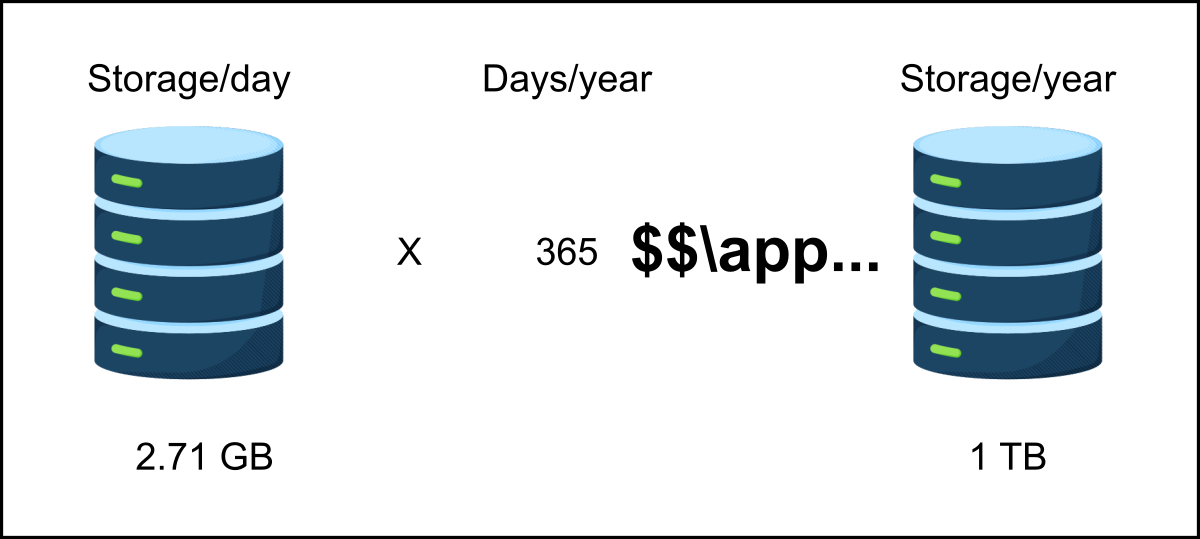
\includegraphics[width=0.5\textwidth]{Images/chapter_30/section_6376322179268608/6415432734343168.png}
 \caption{Total storage required by Uber in an year}
\end{figure}

\begin{quote}
\textbf{Note:} We can adjust the values in the table to see how the estimations change.
\end{quote}
\subsubsection{Bandwidth estimation}\label{9IotzVVNwsEUc19_vO_-U}
\\
We'll only consider drivers' location updates and trip data for bandwidth calculation since other factors don't require significant bandwidth. We have 20 million daily rides, which means we have approximately 232 trips per second.

\[
\frac{20,000,000}{86,400} \approx 232\ \text{trips per second}
\]

Now, each trip takes around 100 Bytes. So, it takes around 23 KB per second of bandwidth.

\[
232 \times 100 = 23,200\ \text{bytes} = 23\ \text{KB} \times 8 = 185\ \text{kbps}
\]

\hfill\break
As already stated, the driver's location is updated every four seconds. If we receive the driver's ID (3 Bytes) and location (16 Bytes), our application will take the following bandwidth:

\[
3M\ \text{active drivers} \times (3 + 16)B = 57\ \text{MB} \times 8 = \frac{456}{4} = 114\ \text{Mbps}
\]

\textbf{Note:} To optimize bandwidth, the system should push updates only to relevant nearby riders using spatial partitioning, like QuadTree or geohash-based sharding. For trip notifications, while 232 trips/sec is the average, peak loads may require burst handling.
\\
These bandwidth requirements are modest because we didn't include bandwidth needs for maps and other components that are present in the real Uber service.


\begin{figure}[htbp]
 \centering
 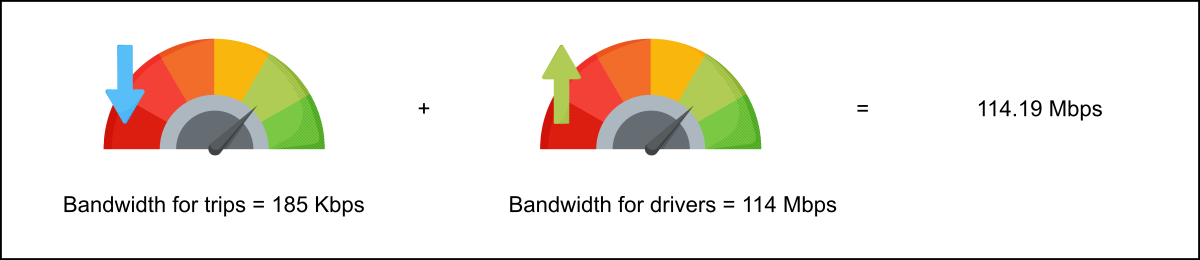
\includegraphics[width=0.5\textwidth]{Images/chapter_30/section_6376322179268608/5376394060496896.png}
 \caption{The total bandwidth required by Uber}
\end{figure}

\begin{quote}
\textbf{Note:} We can adjust the values in the table to see how the requirements change.
\end{quote}
\\
We've ignored the bandwidth from the Uber service to users because it was very small. More bandwidth will be required for sending map data from the Uber service to users, which we've also discussed in the \href{https://www.educative.io/courses/grokking-the-system-design-interview/system-design-google-maps}{Google Maps} chapter.

\subsubsection{Number of servers estimation}\label{pIUauht-fGe9gs0L7d5Hj}
\\
Suppose we have 20 million daily active riders and three million daily active drivers, totaling 23 million daily active users. Considering
\href{https://www.educative.io/courses/grokking-the-system-design-interview/put-back-of-the-envelope-numbers-in-perspective}{our assumption} of using daily active users as a proxy for the number of requests per second in peak load times, we get 23 million requests per second. Then
, we use the following formula to calculate the number of servers:

\[
\text{Servers needed at peak load = } \frac{\text{Number of requests/second}}{\text{RPS of server}}
\]

Using 64,000 as an estimated RPS a server can handle, the required servers are estimated as follows:

\[
\text{Servers needed at peak load} = \frac{23\ \text{million}}{64,000} \approx 360\ \text{servers}
\]

\begin{figure}[htbp]
 \centering
 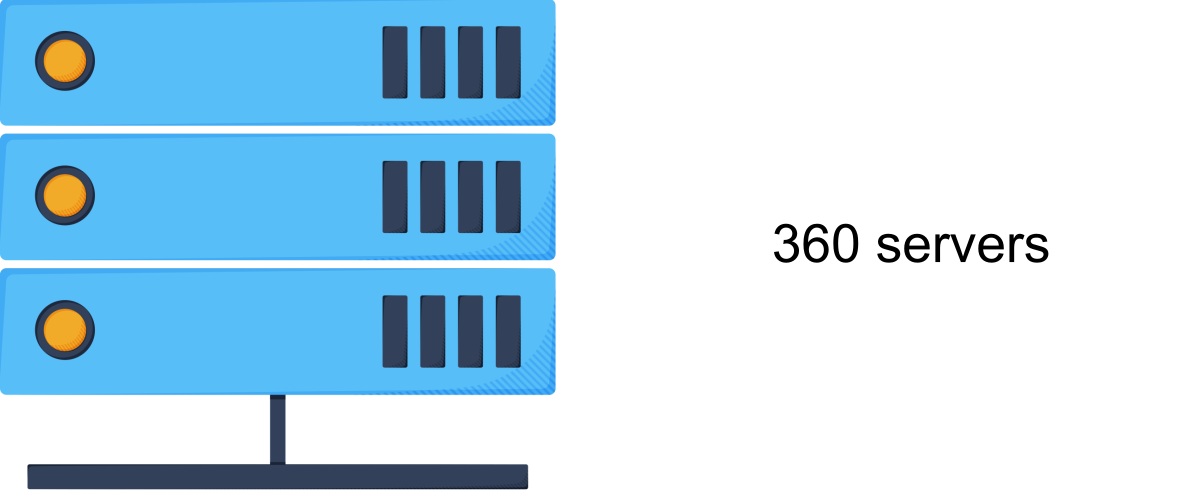
\includegraphics[width=0.5\textwidth]{Images/chapter_30/section_6376322179268608/4852892576382976.png}
 \caption{The number of servers required for Uber service}
\end{figure}

\subsection{Building blocks we will use}\label{4DvcpHlcCERI64PRAUOAU}
\\
The design of Uber utilizes the following building blocks:

\begin{figure}[htbp]
 \centering
 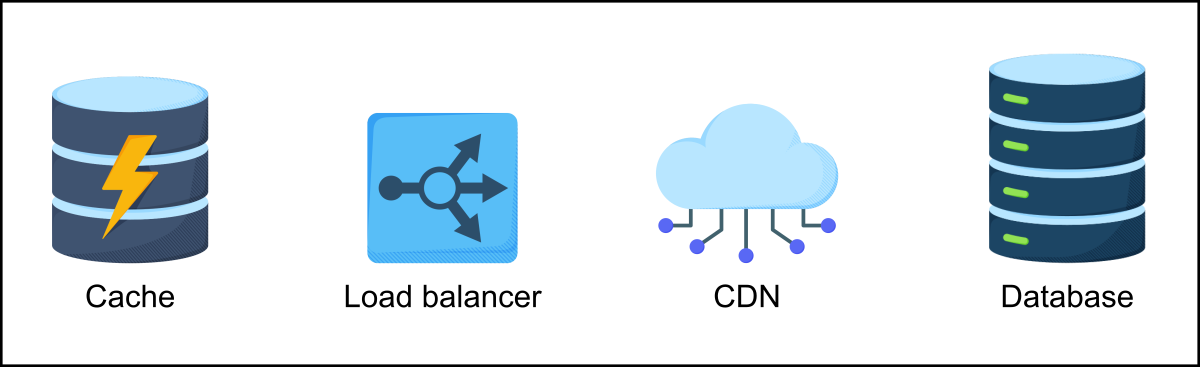
\includegraphics[width=0.5\textwidth]{Images/chapter_30/section_6376322179268608/5052928933363712.png}
 \caption{Building blocks in the high-level design of Uber}
\end{figure}

\begin{itemize}
\item
\protect\phantomsection\label{Hd4RUNSHghUOE1oDRityk}
\href{https://www.educative.io/courses/grokking-the-system-design-interview/system-design-the-distributed-cache}{\textbf{A cache}} stores the most requested data for quick responses.
\item
\protect\phantomsection\label{ZxphwU_Ud98lMaXN7ixD2}
\href{https://www.educative.io/courses/grokking-the-system-design-interview/introduction-to-load-balancers}{\textbf{A load balancer}} distributes the read/write requests among the respective services.
\item
\protect\phantomsection\label{m__q9RBRpwLRNN2t2tXyk}
\href{https://www.educative.io/courses/grokking-the-system-design-interview/system-design-the-content-delivery-network-cdn}{\textbf{CDNs}} are used to effectively deliver content to end users, reducing delay and the burden on end-servers.
\item
\protect\phantomsection\label{LI9FGitNUEj2veIQ2NMGk}
\href{https://www.educative.io/courses/grokking-the-system-design-interview/introduction-to-databases}{\textbf{Databases}} store the metadata of riders, drivers, and trips.
\end{itemize}
\\
Riders' and drivers' devices should have sufficient bandwidth and GPS equipment for smooth navigation with maps.
\begin{quote}
\textbf{Note:} The information provided in this chapter is inspired by the engineering blog of Uber.
\end{quote}

% End of section content